\documentclass{article}
\usepackage{pgfplots}
\usepgfplotslibrary{groupplots,dateplot}
\usetikzlibrary{patterns,shapes.arrows}
\pgfplotsset{compat=newest}
\usepackage{tikz}
\usetikzlibrary{shapes, arrows.meta, positioning}
\usepackage[utf8]{inputenc}
\usepackage{amsmath}
\usepgfplotslibrary{groupplots}
\usepgfplotslibrary{fillbetween}
\usetikzlibrary{arrows,decorations.pathmorphing,positioning,fit,trees,shapes,shadows,automata,calc}
\usetikzlibrary{patterns,arrows,arrows.meta,calc,shapes,shadows,decorations.pathmorphing,decorations.pathreplacing,automata,shapes.multipart,positioning,shapes.geometric,fit,circuits,trees,shapes.gates.logic.US,fit, matrix,arrows.meta, quotes}
\usetikzlibrary{backgrounds,scopes}

\begin{document}

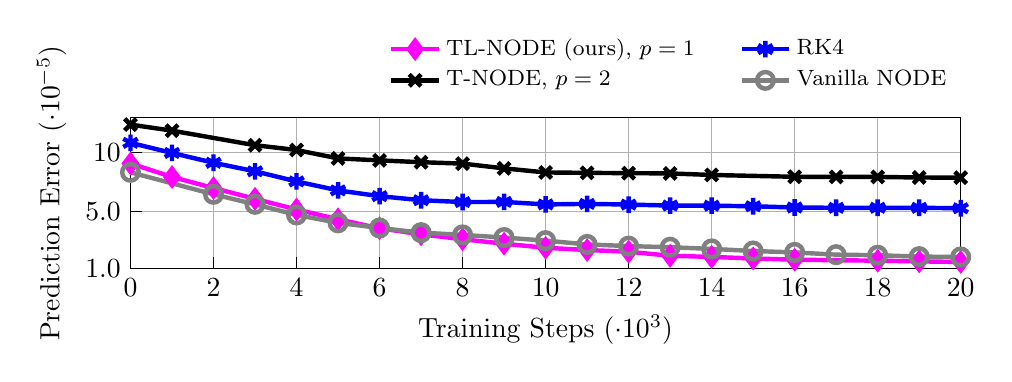
\begin{tikzpicture}

\definecolor{color0}{rgb}{1,0.647058823529412,0}
\definecolor{color1}{rgb}{1,0,1}

\begin{axis}[
height=3.5cm,
width=\columnwidth,
legend cell align={left},
legend columns = 2,
legend style={
    /tikz/every even column/.append style={column sep=0.5cm},
    font=\footnotesize, 
    fill opacity=0.8, 
    draw opacity=1, 
    text opacity=1, 
    draw=none,
    at={(1.0, 1.6)},
    },
tick align=inside,
tick pos=left,
x grid style={white!69.0196078431373!black},
xlabel={Training Steps \((\cdot 10^3)\)},
xmajorgrids,
xmin=0, xmax=20,
xtick style={color=black},
y grid style={white!69.0196078431373!black},
ylabel={Prediction Error \((\cdot10^{-5})\)},
ymajorgrids,
ymin=9.64840992828882e-07, ymax=0.000129321379371469,
ytick style={color=black},
ytick={0.000001, 0.00005, 0.0001},
yticklabels={1.0, 5.0, 10},
scaled y ticks=false
]

\addplot [ultra thick, color1, mark=diamond*, mark size=3, mark options={solid}]
table {%
0 9.0479850769043e-05
1 7.9035758972168e-05
2 6.96182250976562e-05
3 6.04391098022461e-05
4 5.13792037963867e-05
5 4.3034553527832e-05
6 3.5405158996582e-05
7 3.02791595458984e-05
8 2.61068344116211e-05
9 2.22921371459961e-05
10 1.88350677490234e-05
11 1.69277191162109e-05
12 1.54972076416016e-05
13 1.20401382446289e-05
14 1.10864639282227e-05
15 9.77516174316406e-06
16 8.70227813720703e-06
18 7.86781311035156e-06
19 7.27176666259766e-06
20 6.79492950439453e-06
};
\addlegendentry{TL-NODE (ours), \(p=1\)}
% 0 9.10758972167969e-05
% 1 8.13007354736328e-05
% 2 7.15255737304688e-05
% 3 6.23464584350586e-05
% 4 5.43594360351562e-05
% 5 4.58955764770508e-05
% 6 3.86238098144531e-05
% 7 3.40938568115234e-05
% 8 3.01599502563477e-05
% 9 2.65836715698242e-05
% 10 2.30073928833008e-05
% 11 2.11000442504883e-05
% 12 1.95503234863281e-05
% 13 1.6331672668457e-05
% 14 1.68085098266602e-05
% 15 1.62124633789062e-05
% 16 1.50203704833984e-05
% 17 1.51395797729492e-05
% 18 1.57356262207031e-05
% 19 1.56164169311523e-05
% 20 1.56164169311523e-05

\addplot [ultra thick, blue, mark=asterisk, mark size=3, mark options={solid}]
table {%
0 0.000108003616333008
1 9.94205474853516e-05
2 9.10758972167969e-05
3 8.38041305541992e-05
4 7.5221061706543e-05
5 6.7591667175293e-05
6 6.27040863037109e-05
7 5.92470169067383e-05
8 5.76972961425781e-05
9 5.78165054321289e-05
10 5.56707382202148e-05
11 5.6147575378418e-05
12 5.55515289306641e-05
13 5.47170639038086e-05
14 5.45978546142578e-05
15 5.41210174560547e-05
16 5.30481338500977e-05
17 5.28097152709961e-05
18 5.28097152709961e-05
19 5.28097152709961e-05
20 5.24520874023438e-05
};
\addlegendentry{RK4}
% 0 0.000109195709228516
% 1 0.00010073184967041
% 2 9.2625617980957e-05
% 3 8.54730606079102e-05
% 4 7.70092010498047e-05
% 5 6.96182250976562e-05
% 6 6.47306442260742e-05
% 7 6.13927841186523e-05
% 8 5.9962272644043e-05
% 9 6.02006912231445e-05
% 10 5.8293342590332e-05
% 11 5.86509704589844e-05
% 12 5.81741333007812e-05
% 13 5.74588775634766e-05
% 14 5.73396682739258e-05
% 15 5.69820404052734e-05
% 16 5.62667846679688e-05
% 17 5.59091567993164e-05
% 19 5.57899475097656e-05
% 20 5.54323196411133e-05

\addplot [ultra thick, black, mark=x, mark size=3, mark options={solid}]
table {%
0 0.000123500823974609
1 0.000118374824523926
3 0.000105977058410645
4 0.000101923942565918
5 9.47713851928711e-05
6 9.31024551391602e-05
7 9.1552734375e-05
8 9.03606414794922e-05
9 8.63075256347656e-05
10 8.2850456237793e-05
11 8.24928283691406e-05
12 8.22544097900391e-05
13 8.20159912109375e-05
14 8.07046890258789e-05
16 7.91549682617188e-05
17 7.9035758972168e-05
18 7.9035758972168e-05
19 7.85589218139648e-05
20 7.84397125244141e-05
};
\addlegendentry{T-NODE, \(p=2\)}
% 0 0.000117897987365723
% 1 0.000112533569335938
% 3 9.97781753540039e-05
% 4 9.56058502197266e-05
% 5 8.82148742675781e-05
% 6 8.6665153503418e-05
% 7 8.53538513183594e-05
% 8 8.44001770019531e-05
% 9 8.14199447631836e-05
% 10 7.87973403930664e-05
% 11 7.84397125244141e-05
% 12 7.83205032348633e-05
% 13 7.80820846557617e-05
% 14 7.70092010498047e-05
% 16 7.58171081542969e-05
% 17 7.56978988647461e-05
% 18 7.56978988647461e-05
% 19 7.5221061706543e-05
% 20 7.5221061706543e-05

\addplot [ultra thick, white!50.1960784313725!black, mark=o, mark size=3, mark options={solid}]
table {%
0 8.29696655273438e-05
2 6.42538070678711e-05
3 5.57899475097656e-05
4 4.67300415039062e-05
5 4.00543212890625e-05
6 3.56435775756836e-05
7 3.17096710205078e-05
8 2.98023223876953e-05
9 2.75373458862305e-05
10 2.49147415161133e-05
11 2.16960906982422e-05
12 2.02655792236328e-05
13 1.93119049072266e-05
14 1.78813934326172e-05
15 1.60932540893555e-05
16 1.49011611938477e-05
17 1.29938125610352e-05
18 1.2516975402832e-05
19 1.13248825073242e-05
20 1.10864639282227e-05
21 1.06096267700195e-05
22 1.02519989013672e-05
24 9.89437103271484e-06
25 9.41753387451172e-06
27 9.05990600585938e-06
28 8.70227813720703e-06
31 8.22544097900391e-06
32 8.10623168945312e-06
34 7.86781311035156e-06
35 7.74860382080078e-06
37 7.51018524169922e-06
40 7.39097595214844e-06
};
\addlegendentry{Vanilla NODE}
\end{axis}

\end{tikzpicture}

\end{document}